\section{Anhang}
\addtocontents{toc}{\protect\setcounter{tocdepth}{-1}}

\subsection{XML}
\label{xml}
\vspace{-5px}
	\begin{spacing}{0.75}
		\begin{xmlcode}[firstnumber=1]
<?xml version="1.0" encoding="UTF-8"?><ShortcutTestResultModel name="chrome-WINDOWS">
  <browserName>chrome</browserName>
  <browserVersion>66.0.3359.170</browserVersion>
  <osName>Windows 10</osName>
  <osVersion>10.0</osVersion>
  <failedShortcuts>
    <ShortcutTestEntryModel name="e5e6edfc-6f2c-4762-8242-3887f61699c4">
      <shortcut>
        <keyModifiers>
          <KeyModifierDataModel name="SHIFT">
            <keyModifier>SHIFT</keyModifier>
          </KeyModifierDataModel>
          <KeyModifierDataModel name="ALT">
            <keyModifier>ALT</keyModifier>
          </KeyModifierDataModel>
          <KeyModifierDataModel name="CTRL">
            <keyModifier>CTRL</keyModifier>
          </KeyModifierDataModel>
        </keyModifiers>
        <key>A</key>
      </shortcut>
      <success>true</success>
    </ShortcutTestEntryModel>
    <ShortcutTestEntryModel name="95d83f77-be27-4b1c-b0a8-bd0cfb07c0a4">
      <shortcut>
        <keyModifiers>
          <KeyModifierDataModel name="SHIFT">
            <keyModifier>SHIFT</keyModifier>
          </KeyModifierDataModel>
          <KeyModifierDataModel name="META">
            <keyModifier>META</keyModifier>
          </KeyModifierDataModel>
        </keyModifiers>
        <key>INSERT</key>
      </shortcut>
      <success>true</success>
    </ShortcutTestEntryModel>
    <ShortcutTestEntryModel name="cccd89e4-02bd-4638-9220-6d7e2bc9815a">
      <shortcut>
        <keyModifiers>
          <KeyModifierDataModel name="ALT_GRAPH">
            <keyModifier>ALT_GRAPH</keyModifier>
          </KeyModifierDataModel>
          <KeyModifierDataModel name="ALT">
            <keyModifier>ALT</keyModifier>
          </KeyModifierDataModel>
          <KeyModifierDataModel name="CTRL">
            <keyModifier>CTRL</keyModifier>
          </KeyModifierDataModel>
        </keyModifiers>
        <key>NUM0</key>
      </shortcut>
      <success>true</success>
    </ShortcutTestEntryModel>
    <ShortcutTestEntryModel name="3afd18fa-8f23-46aa-bd80-ca3a331fa677">
      <shortcut>
        <keyModifiers>
          <KeyModifierDataModel name="ALT_GRAPH">
            <keyModifier>ALT_GRAPH</keyModifier>
          </KeyModifierDataModel>
          <KeyModifierDataModel name="SHIFT">
            <keyModifier>SHIFT</keyModifier>
          </KeyModifierDataModel>
          <KeyModifierDataModel name="CTRL">
            <keyModifier>CTRL</keyModifier>
          </KeyModifierDataModel>
          <KeyModifierDataModel name="META">
            <keyModifier>META</keyModifier>
          </KeyModifierDataModel>
        </keyModifiers>
        <key>F10</key>
      </shortcut>
      <success>true</success>
    </ShortcutTestEntryModel>
    ...
\end{xmlcode}
\end{spacing}
\subsection{Verwendete Ressourcen}
\label{ressources}

\textbf{Hardware}

\begin{itemize}
\item Büroarbeitsplatz (PC, Tastatur, Maus etc.)
\end{itemize}
 
\textbf{Software}

\begin{itemize}
\item Windows 10 Professional – Betriebssystem
\item IntelliJ IDEA – Entwicklungsumgebung Java
\item Java JDK - Software Developer Kit (SDK)
\item Maven - Buildsystem
\item git – Verteilte Versionsverwaltung
\item MiKTeX – Distribution des Textsatzsystems \LaTeX
\item TeXstudio – Entwicklungsumgebung für \TeX
\item yEd Graph Editor - Anwendung zur Erstellung von UML-Diagramme
\end{itemize}

\textbf{Personal}

\begin{itemize}
\item Mitarbeiter der UX-Abteilung – Erstellung von Designentwürfen
\item Entwickler – Umsetzung des Projektes
\end{itemize}

\subsection{Anwendungsfälle}
\label{usecase}

\begin{figure}[H]
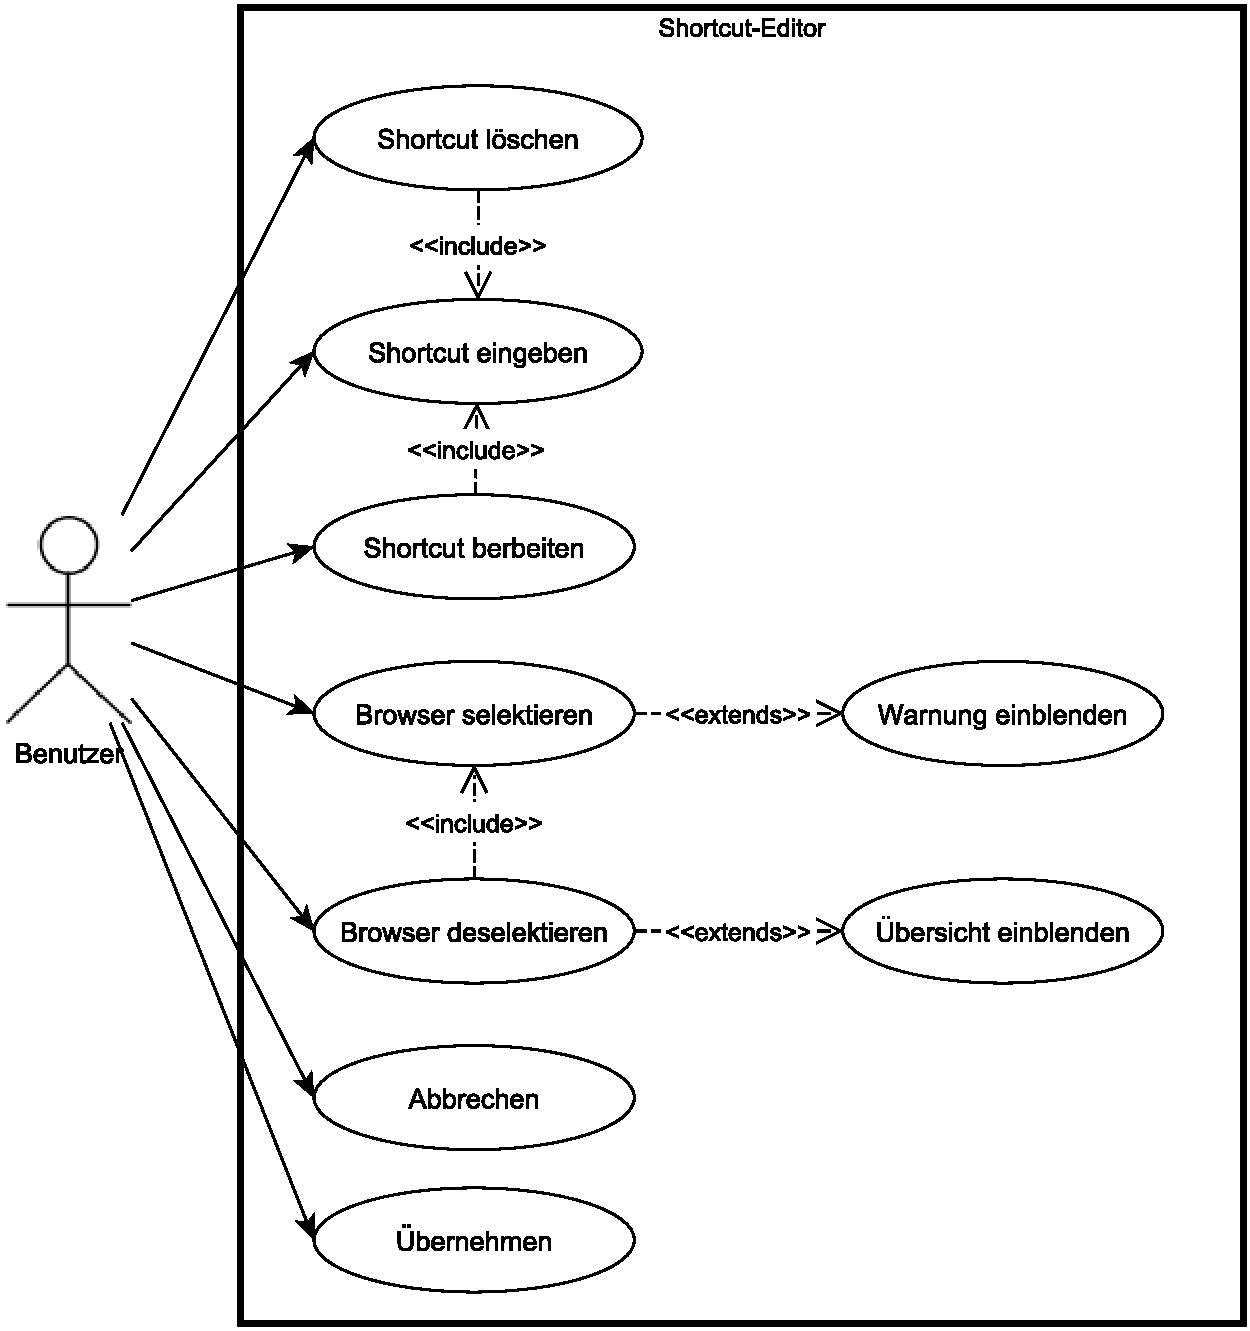
\includegraphics[width=\linewidth]{../graphic/diagrams/UC_Anwendungsfall/Anwendungsfall}
\end{figure}

\subsection{Zeichnen des Icons im CheckToggleButton}
\label{CheckToggleButton}
\begin{spacing}{0.75}
\begin{javacode}[firstnumber=20]
  
  /**
  * Aktualisiert das Icon
  */
  private void _updateIcon()
  {
    int width = icon.getWidth(null);
    int height = icon.getHeight(null);
    
    Image stateIcon = checked ? checkedIcon : uncheckedIcon;
    
    int x2 = width - stateIcon.getWidth(null);
    int y2 = height - stateIcon.getHeight(null);
    
    BufferedImage image = new BufferedImage(width, height, BufferedImage.TYPE_INT_ARGB);
    
    Graphics g = image.getGraphics();
    
    g.drawImage(icon, 0, 0, null);
    g.drawImage(stateIcon, x2, y2, null);
    
    setIcon(new ImageIcon(image));
  }
\end{javacode}
\end{spacing}

\subsection{CheckItemButton}
\label{CheckItemButton}
\begin{spacing}{0.75}
\begin{javacode}[firstnumber=12]
public class CheckItemButton extends CheckToggleButton
{
  private final ICheckItem checkItem;
  
  /**
  * Konstruktor
  *
  * @param pCheckItem CheckItem
  */
  public CheckItemButton(ICheckItem pCheckItem)
  {
    super(pCheckItem.getIcon().getImage());
    
    checkItem = pCheckItem;
    
    setChecked(checkItem.isSuccessful());
    setToolTipText(checkItem.getType());
    setPreferredSize(IShortcutEditorConstants.CHECK_ITEM_SIZE);
    setMinimumSize(IShortcutEditorConstants.CHECK_ITEM_SIZE);
    setMaximumSize(IShortcutEditorConstants.CHECK_ITEM_SIZE);
    setOpaque(true);
  }
  
  /**
  * Gibt das zugehörige ICheckItem zurück
  *
  * @return zugehörige ICheckItem
  */
  public ICheckItem getCheckItem()
  {
    return checkItem;
  }
}

\end{javacode}
\end{spacing}

\subsection{Setzen der CheckItems im CheckItemContainer}
\label{CheckItemContainer}
\begin{spacing}{0.75}
\begin{javacode}[firstnumber=43]
/**
* Setzt die zu visualisierenden ICheckItems
*
* @param pCheckItems zu visualisierenden ICheckItems
*/
public void setCheckItems(ICheckItem[] pCheckItems)
{
  ICheckItem selection = getSelection();
  
  for (CheckItemButton comp : getAllCheckButtons())
  {
    comp.removeItemListener(itemListener);
    removeCheckButton(comp);
  }
  
  if(pCheckItems != null)
  {
    for (ICheckItem item : pCheckItems)
    {
      CheckItemButton component = new CheckItemButton(item);
      component.addItemListener(itemListener);
      addCheckButton(component);
    }
  }
  
  revalidate();
  repaint();
}

\end{javacode}
\end{spacing}

\subsection{ShortcutStructureTable}
\label{ShortcutStructureTable}
\begin{spacing}{0.75}
\begin{javacode}[firstnumber=25]
public class ShortcutStructureTable extends JPanel implements IShortcutStructureView
{
  private SplitsTreeTable table;
  private ShortcutStructureTreeModel treeModel;
  
  private ShortcutStructureModel model;
  
  /**
  * Konstruktor
  */
  public ShortcutStructureTable()
  {
    setLayout(new BorderLayout());
    
    model = new ShortcutStructureModel();
    
    table = new SplitsTreeTable();
    table.setRootVisible(false);
    table.setRenderDataProvider(new _ModelProvider());
    table.setShowVerticalLines(false);
    table.setShowHorizontalLines(false);
    table.setSelectionMode(ListSelectionModel.SINGLE_SELECTION);
    table.setRowHeight(IShortcutEditorConstants.TABLE_ROW_HEIGHT);
    
    add(new JScrollPane(table), BorderLayout.CENTER);
  }
  
  @Override
  public IEditorShortcutNode getRootShortcutNode()
  {
    return model.getRootShortcutNode();
  }
  
  @Override
  public void setNodePath(AditoTreePath<IEditorShortcutNode> pPath)
  {
    model.setNodePath(pPath);
  }

...

\end{javacode}
\end{spacing}

\subsection{ShortcutPathComponent}
\label{ShortcutPathComponent}
\begin{figure}
  \begin{spacing}{0.75}
    \begin{javacode}[firstnumber=19]
public class ShortcutPathComponent extends JPanel implements IShortcutStructureView
{
  private static final int GAP = 5;
  
  private BreadCrumb<IEditorShortcutNode> breadCrumb;
  
  /**
  * Konstruktor
  */
  public ShortcutPathComponent()
  {
    double[] x = {TableLayout.PREFERRED, GAP, TableLayout.MINIMUM};
    double[] y = {TableLayout.PREFERRED};
    
    setLayout(new TableLayout(x, y));
    
    TableLayoutUtil tlu = new TableLayoutUtil(this);
    
    JLabel textLabel = new JLabel(IShortcutEditorConstants.TEXT_SHORTCUT_FOR);
    tlu.add(0, 0, textLabel);
    
    breadCrumb = new BreadCrumb<>();
    tlu.add(2, 0, breadCrumb);
  }
  
  @Override
  public void setRootShortcutNode(IEditorShortcutNode pNode)
  {
    breadCrumb.setRootNode(pNode);
    
    synchronized (nodeChangeListeners)
    {
      for (INodeChangeListener listener : nodeChangeListeners)
      listener.groupChanged(pNode);
    }
  }
  
  @Override
  public IEditorShortcutNode getRootShortcutNode()
  {
    return breadCrumb.getRootNode();
  }
  
  @Override
  public void setNodePath(AditoTreePath<IEditorShortcutNode> pPath)
  {
    breadCrumb.setPath(pPath);
  }
  
  @Override
  public AditoTreePath<IEditorShortcutNode> getNodePath()
  {
    return breadCrumb.getPath();
  }
  
  @Override
  public void addPathChangeListener(IAditoPathChangeListener<IEditorShortcutNode> 
                                    pChangeListener)
  {
    breadCrumb.addPathChangeListener(pChangeListener);
  }
  
  @Override
  public void removePathChangeListener(IAditoPathChangeListener<IEditorShortcutNode> 
                                       pChangeListener)
  {
    breadCrumb.removePathChangeListener(pChangeListener);
  }

...

\end{javacode}
\end{spacing}
\end{figure}

\subsection{ShortcutEditorUI}
\label{ShortcutEditorUI}

  \begin{spacing}{0.75}
    \begin{javacode}[firstnumber=25]
public class ShortcutEditorUI extends JPanel implements IShortcutEditorUI
{
  private ShortcutField shortcutField;
  private CheckItemContainer checkContainer;
  private CheckItemAccordion checkAccordion;
  
  private ShortcutStructureModel model;
  
  private static final int GAP = 5;
  
  /**
  * Konstruktor
  */
  public ShortcutEditorUI()
  {
    double[] x = {10, TableLayout.FILL, 10};
    double[] y = {GAP,
                  20,
                  GAP,
                  80,
                  GAP,
                  50,
                  GAP,
                  TableLayout.FILL,
                  10};
    
    setLayout(new TableLayout(x, y));
    
    TableLayoutUtil tlu = new TableLayoutUtil(this);
    
    model = new ShortcutStructureModel();
    
    ShortcutPathComponent pathComp = new ShortcutPathComponent();
    ShortcutStructureTable modelViewer = new ShortcutStructureTable();
    
    new ShortcutStructurePresenter(model, pathComp, modelViewer);
    
    shortcutField = new ShortcutField();
    checkAccordion = new CheckItemAccordion();
    checkContainer = checkAccordion.getRootCheckItemContainer();
    
    tlu.add(1, 1, pathComp);
    tlu.add(1, 3, shortcutField);
    tlu.add(1, 5, checkContainer);
    tlu.add(1, 7, checkAccordion);
    tlu.add(1, 7, modelViewer);
  }
  
  public void setShortcut(IShortcut pShortcut)
  {
    shortcutField.setShortcut(pShortcut);
  }
  
  public IShortcut getShortcut()
  {
    return shortcutField.getShortcut();
  }

  public void addShortcutChangeListener(IShortcutChangeListener pChangeListener)
  {
    shortcutField.addShortcutChangeListener(pChangeListener);
  }

  public void removeShortcutChangeListener(IShortcutChangeListener pChangeListener)
  {
    shortcutField.removeShortcutChangeListener(pChangeListener);
  }

  public void setCheckItemGroup(ICheckItemGroup pRootGroup)
  {
    checkAccordion.setCheckItemGroup(pRootGroup);
  }

  @Override
  public ICheckItemGroup getCheckItemGroup()
  {
    return checkAccordion.getCheckItemGroup();
  }

...
\end{javacode}
\end{spacing}

\subsection{ShortcutEditorPresenter}
\label{ShortcutEditorPresenter}
\vspace{-5px}
  \begin{spacing}{0.75}
    \begin{javacode}[firstnumber=19]
public class ShortcutEditorPresenter
{
  private final IShortcutEditorUI ui;
  private final IShortcutEditorStore editorStore;
  private final IShortcutChangeListener shortcutChangeListener;
  private IEditorShortcutModel currModel;
  
  /**
  * @param pUi zu steuernde UI
  * @param pStore Store zum beziehen der Daten
  */
  public ShortcutEditorPresenter(IShortcutEditorUI pUi, IShortcutEditorStore pStore)
  {
    ui = pUi;
    editorStore = pStore;
    
    shortcutChangeListener = new _ShortcutListener();
    
    ui.addShortcutChangeListener(shortcutChangeListener);
    ui.addPathChangeListener(new _PathListener());
    ui.setRootShortcutNode(pStore.getShortcutModelRootNode());
  }
  
  /**
  * Extrahiert aus dem Pfad das ShortcutModel, auf welchen sich der Pfad bezieht
  *
  * @param pPath Pfad zum Model
  * @return ShortcutModel
  */
  private IEditorShortcutModel _getShortcutModel(AditoTreePath<IEditorShortcutNode> pPath)
  {
    AditoTreePath<IEditorShortcutNode> node = pPath;
    
    while (node != null && !(node.getNode() instanceof IEditorShortcutModel))
      node = node.getNext();
    
    if(node == null)
      return null;
    
    return (IEditorShortcutModel) node.getNode();
  }
  
  /**
  * Listener zum handeln von Pfadänderungen
  */
  private class _PathListener implements IAditoPathChangeListener<IEditorShortcutNode>
  {
    @Override
    public void pathChange(AditoTreePath<IEditorShortcutNode> pPath)
    {
      if(currModel != null)
        currModel.removeShortcutChangeListener(shortcutChangeListener);
      
      currModel = _getShortcutModel(pPath);
      
      if (currModel != null)
      {
        currModel.addShortcutChangeListener(shortcutChangeListener);
        ui.setShortcut(currModel.getShortcut());
      }
    }
  }
  /**
  * Listener zum handeln von Shortcutänderungen
  */
  private class _ShortcutListener implements IShortcutChangeListener
  {
    @Override
    public void shortcutChanged(IShortcut pShortcut)
    {
      if (!Objects.equals(pShortcut, ui.getShortcut()))
        ui.setShortcut(pShortcut);
      
      if (currModel != null && !Objects.equals(pShortcut, currModel.getShortcut()))
        currModel.setShortcut(pShortcut);
      
      ICheckItemGroup rootCheckItem = editorStore.getRootCheckItem(pShortcut);
      ui.setCheckItemGroup(rootCheckItem);
    }
  }
}
\end{javacode}
\end{spacing}

\subsection{ShortcutStructurePresenter}
\label{ShortcutStructurePresenter}
\vspace{-5px}
  \begin{spacing}{0.75}
    \begin{javacode}[firstnumber=21]
public class ShortcutStructurePresenter
{
  private final INodeChangeListener groupChangeListener;
  private final IAditoPathChangeListener<IEditorShortcutNode> pathChangeListener;
  
  private final ShortcutStructureModel model;
  private final List<IShortcutStructureView> views;
  
  /**
  * Konstruktor
  *
  * @param pModel Das Hauptmodel
  * @param pViews belibige Anzahl von Views
  */
  public ShortcutStructurePresenter(ShortcutStructureModel pModel, 
                                    IShortcutStructureView... pViews)
  {
    model = pModel;
    views = new ArrayList<>();
    
    groupChangeListener = new _NodeChangeListener();
    pathChangeListener = new _PathChangeListener();
    
    model.addPathChangeListener(this::_updatePath);
    model.addNodeChangeListener(this::_updateGroup);
    
    if(pViews != null)
    for (IShortcutStructureView view : pViews)
    addView(view);
  }
  
  /**
  * Fügt dem Presenter eine View hinzu
  *
  * @param pView hinzuzufügende View
  */
  public void addView(IShortcutStructureView pView)
  {
    synchronized (views)
    {
      views.add(pView);
    }
    
    pView.addPathChangeListener(pathChangeListener);
    pView.addNodeChangeListener(groupChangeListener);
    
    pView.setRootShortcutNode(model.getRootShortcutNode());
    pView.setNodePath(model.getNodePath());
  }
  
  /**
  * Entfernt eine View
  *
  * @param pView zu entfernende View
  */
  public void removeView(IShortcutStructureView pView)
  {
    synchronized (views)
    {
      views.remove(pView);
    }
    
    pView.removePathChangeListener(pathChangeListener);
    pView.removeNodeChangeListener(groupChangeListener);
  }
  
  /**
  * Aktualisiert die ShortcutModels in den einzelenen Views
  *
  * @param pGroup zu sentzende Gruppe mit ShortcutModels
  */
  private void _updateGroup(IEditorShortcutNode pGroup)
  {
    synchronized (views)
    {
      for (IShortcutStructureView view : views)
      if (!Objects.equals(view.getRootShortcutNode(), pGroup))
      view.setRootShortcutNode(pGroup);
    }
  }
\end{javacode}
\end{spacing}
\vspace{-5px}
  \begin{spacing}{0.75}
    \begin{javacode}[firstnumber=100]
  
  /**
  * Aktualisiert den Pfad in den einzelen Views
  *
  * @param pPath zu setztender Pfad
  */
  private void _updatePath(AditoTreePath<IEditorShortcutNode> pPath)
  {
    synchronized (views)
    {
      for (IShortcutStructureView view : views)
      if (!Objects.equals(view.getNodePath(), pPath))
      view.setNodePath(pPath);
    }
  }
  
  /**
  * Listener, welcher Änderungen der ShortcutGroup in das Hauptmodel überträgt
  */
  private class _ShortcutNodeChangeListener implements INodeChangeListener
  {
    @Override
    public void groupChanged(IEditorShortcutNode pNode)
    {
      if (!Objects.equals(model.getRootShortcutNode(), pNode))
      model.setRootShortcutNode(pNode);
    }
  }
  
  /**
  * Listener, welcher Änderungen der ShortcutPath in das Hauptmodel überträgt
  */
  private class _ShortcutPathChangeListener 
                implements IAditoPathChangeListener<IEditorShortcutNode>
  {
    @Override
    public void pathChange(AditoTreePath<IEditorShortcutNode> pPath)
    {
      if (!Objects.equals(model.getNodePath(), pPath))
      model.setNodePath(pPath);
    }
  }
}
\end{javacode}
\end{spacing}

\subsection{ShortcutStructureModel}
\label{ShortcutStructureModel}
\vspace{-5px}
  \begin{spacing}{0.75}
    \begin{javacode}[firstnumber=21]
public class ShortcutStructureModel implements IShortcutStructureView
{
  private final List<IAditoPathChangeListener<IEditorShortcutNode>> 
       pathChangeListeners = new ArrayList<>();
  private final List<INodeChangeListener> nodeChangeListeners = new ArrayList<>();
  
  private IEditorShortcutNode root;
  private AditoTreePath<IEditorShortcutNode> path;
  
  @Override
  public void setRootShortcutNode(IEditorShortcutNode pNode)
  {
    IEditorShortcutNode oldGroup = root;
    
    root = pNode;
    
    if(!Objects.equals(oldGroup, pNode))
     _fireEditorShortcutGroupChangeEvent();
  }
  
  @Override
  public IEditorShortcutNode getRootShortcutNode() { return root; }
  
  @Override
  public void setNodePath(AditoTreePath<IEditorShortcutNode> pPath)
  {
    if(!Objects.equals(path, pPath))
    {
      path = pPath;
      
      _fireEditorShortcutPathChangeEvent();
    }
  }
  
  @Override
  public AditoTreePath<IEditorShortcutNode> getNodePath() { return path; }
  
  @Override
  public void addPathChangeListener(IAditoPathChangeListener<IEditorShortcutNode> 
                                         pChangeListener)
  {
    synchronized (pathChangeListeners)
    {
      pathChangeListeners.add(pChangeListener);
    }
  }
  
  @Override
  public void addNodeChangeListener(INodeChangeListener pChangeListener)
  {
    synchronized (nodeChangeListeners)
    {
      nodeChangeListeners.add(pChangeListener);
    }
  }
  
  /**
  * Feuert ein GroupChangeEvent
  */
  private void _fireEditorShortcutGroupChangeEvent()
  {
    synchronized (nodeChangeListeners)
    {
      for (INodeChangeListener listener : nodeChangeListeners)
       listener.groupChanged(root);
    }
  }
  
  /**
  * Feuert ein PathChangeEvent
  */
  private void _fireEditorShortcutPathChangeEvent()
  {
    synchronized (pathChangeListeners)
    {
      for (IAditoPathChangeListener<IEditorShortcutNode> listener : pathChangeListeners)
       listener.pathChange(path);
    }
  }

...
\end{javacode}
\end{spacing}

\subsection{ShortcutEditor Test}
\label{Test_ShortcutEditor}
\vspace{-12px}
  \begin{spacing}{0.75}
    \begin{javacode}[firstnumber=21]
public class Test_ShortcutEditor
{
  private DialogFixture dialog;
  private ShortcutDummyStore dummyStore;
  private ShortcutEditorUI ui;
  
  @Before
  public void onSetUp()
  {
    _setLookAndFeel();
    
    dummyStore = new ShortcutDummyStore();
    ui = GuiActionRunner.execute(ShortcutEditorUI::new);
    Dialog shortcutDialog = GuiActionRunner.execute(
    () -> ShortcutEditorDialog.createDialog(dummyStore, ui));
    
    dialog = new DialogFixture(shortcutDialog);
    dialog.show();
  }
  
  @Test
  public void test_EnterShortcut()
  {
    int i = 26;
    
    for (IEditorShortcutModel model : dummyStore.getAllModels())
    {
      IShortcut shortcut = new ExtendedShortcut(EKeyModifier.SHIFT, EKey.values()[i++]);
      
      _selectNode(model);
      
      _enterShortcut(shortcut);
      
      Assert.assertEquals(model.getShortcut(), shortcut);
    }
  }
  
  /**
  * Selektiert den übergebenen Node
  * 
  * @param pNode zu selektierender Node
  */
  private void _selectNode(IEditorShortcutNode pNode)
  {
    GuiActionRunner.execute(() -> ui.setNodePath(pNode.getPath()));
    Assert.assertEquals(dialog.table().selectionValue(), pNode.toString());
  }
  
  /**
  * Simuliert die Eingabe eines Shortcuts
  * 
  * @param pShortcut zu simulierender Shortcut
  */
  private void _enterShortcut(IShortcut pShortcut)
  {
    JPanelFixture shortcutField = dialog.panel(SHORTCUT_FIELD_NAME).focus();
    
    SwingShortcut swingShortcut = new SwingShortcut(pShortcut);
    
    List<Integer> keys = swingShortcut.getAllDefaultSpecKeys();
    
    for (Integer i : keys)
    shortcutField.pressKey(i);
    
    for (Integer i : keys)
    shortcutField.releaseKey(i);
    
    Assert.assertEquals(ui.getShortcut(), pShortcut);
  }
  
  private void _setLookAndFeel()
  {
    try
    {
      LookAndFeelSetter.set();
    }
    catch (Exception e)
    {
      throw new RuntimeException(e);
    }
  }
}

\end{javacode}
\end{spacing}
